\section{Reliability}

\subsection{Failure Density, Reliability and Hazard Rate}


\begin{frame}{Definitions}

Suppose $A$ is a black box unit.
\begin{itemize}
	\justifying
	\item \highlightg{Failure density $f_A$}: distribution of the time $T$ that $A$ fails.
	\item \highlightg{Reliability function $R_A$}: the probability that $A$ is working at time $t$, $R_A(t) = 1 - F_A(t)$.
	\item \highlightg{Hazard rate $\rho_A$}: 
	\begin{align*}
	\rho_A(t) & := \lim_{\Delta t \rightarrow 0} \frac{P[t\leq T\leq t + \Delta t|t\leq T]}{\Delta t} \\
	& = \lim_{\Delta t \rightarrow 0} \frac{P[t\leq T\leq t + \Delta t]}{P[T\geq t]\cdot \Delta t} =  \frac{f_A(t)}{R_A(t)}, \\
	R_A(t) & = e^{-\int_0^t \rho_A(x)\U{d}x}.
	\end{align*}
\end{itemize}
One often has information on $\rho_A$, but not $F_A$ or $R_A$.

\end{frame}


\begin{frame}{Series and Parallel Systems}

\begin{itemize}
	\item \structb{Series system with $k$ components.}
	\begin{align*}
	R_s(t) = \prod_{i=1}^k R_i(t),
	\end{align*}
	where $R_i$ is the reliability of the $i$-th component.
	\item \structb{Parallel system with $k$ components.}
	\begin{align*}
	R_p(t) = 1 - \prod_{i=1}^k(1-R_i(t)).
	\end{align*}
\end{itemize}

\end{frame}


\subsection{Weibull Distribution}

\begin{frame}{Weibull Distribution}

\begin{itemize}
	\item \structb{Density function.} $\alpha, \beta > 0$ are parameters,
	\begin{align*}
	f(x) = \left\{
	\begin{array}{ll}
	\alpha\beta x^{\beta-1} e^{-\alpha x^{\beta}}, & x > 0, \\
	0, & \U{otherwise.}
	\end{array}
	\right.
	\end{align*}
	\item \structb{Mean.}
	\begin{align*}
	\mu = \alpha^{-1/\beta} \Gamma(1 + 1/\beta).
	\end{align*}
	\item \structb{Variance.}
	\begin{align*}
	\sigma^2 = \alpha^{-2/\beta} \Gamma(1 + 2/\beta) - \mu^2.
	\end{align*}
\end{itemize}

\end{frame}


\section{Basic Statistics}

\subsection{Samples and Data}


\begin{frame}{Definitions}

\justifying
\begin{itemize}
	\justifying
	\item \highlightg{Statistics} aims to gain information about the parameters of a distribution by conducting experiments.
	\item \highlightg{Population}: a large collection of instances which we want to describe probability.
	\item \highlightg{Random sample of size $n$ from distribution of $X$}: a collection of $n$ independent random variables $X_1, \ldots, X_n$, each with the same distribution as $X$. ($\Leftrightarrow$ $n$ i.i.d. random variables.)
	\item \highlightg{$x$-th percentiles}: $d_x$ such that $x\%$ of values in sampled data are less than or equal to $d_x$. (\highlightg{first, second, third quartile} $\Rightarrow$ $x = 25, 50, 75$.)
	\item \highlightg{Interquartile range}: $\U{IQR} = q_3 - q_1$, measures the dispersion of the data.
	\item \highlightg{Precision}: smallest decimal place of data $\{x_1, \ldots, x_n\}$.
	\item \highlightg{Sample range}: $\max\{x_i\} - \min\{x_i\}$.
\end{itemize}


\end{frame}


\begin{frame}{Visualization --- Histograms}

\structb{Choose bin width / number of bins.}
\begin{itemize}
	\item Sturges's rule.
	\begin{align*}
	k = \lceil \log_2(n)\rceil + 1, \qquad h = \frac{\max\{x_i\} - \min\{x_i\}}{k},
	\end{align*}
	rounding \highlightr{up} to the precision of the data.
	\item Freedman-Diaconis rule.
	\begin{align*}
	h = \frac{2\cdot \U{IQR}}{\sqrt[3]{n}}.
	\end{align*}
\end{itemize}
\structb{Sketch.}
\begin{enumerate}
	\item Choose bin width $h$.
	\item Find minimum of data $\min\{x_i\}$, subtract 1/2 of precision.
	\item Successively add bin width and categorize all the data.
\end{enumerate}

\end{frame}


\begin{frame}{Visualization --- Stem-and-Leaf Diagrams}

\begin{enumerate}
	\justifying
	\item Choose a convenient number of leading decimal digits to serve as stems.
	\item Label the rows using the stems.
	\item For each datum of the random sample, note down the digit following the stem in the corresponding row.
	\item Turn the graph on its side to get an impression of its distribution.
\end{enumerate}

\end{frame}

\begin{frame}{Visualization --- Stem-and-Leaf Diagrams}

\begin{figure}[htbp]
	\centering
	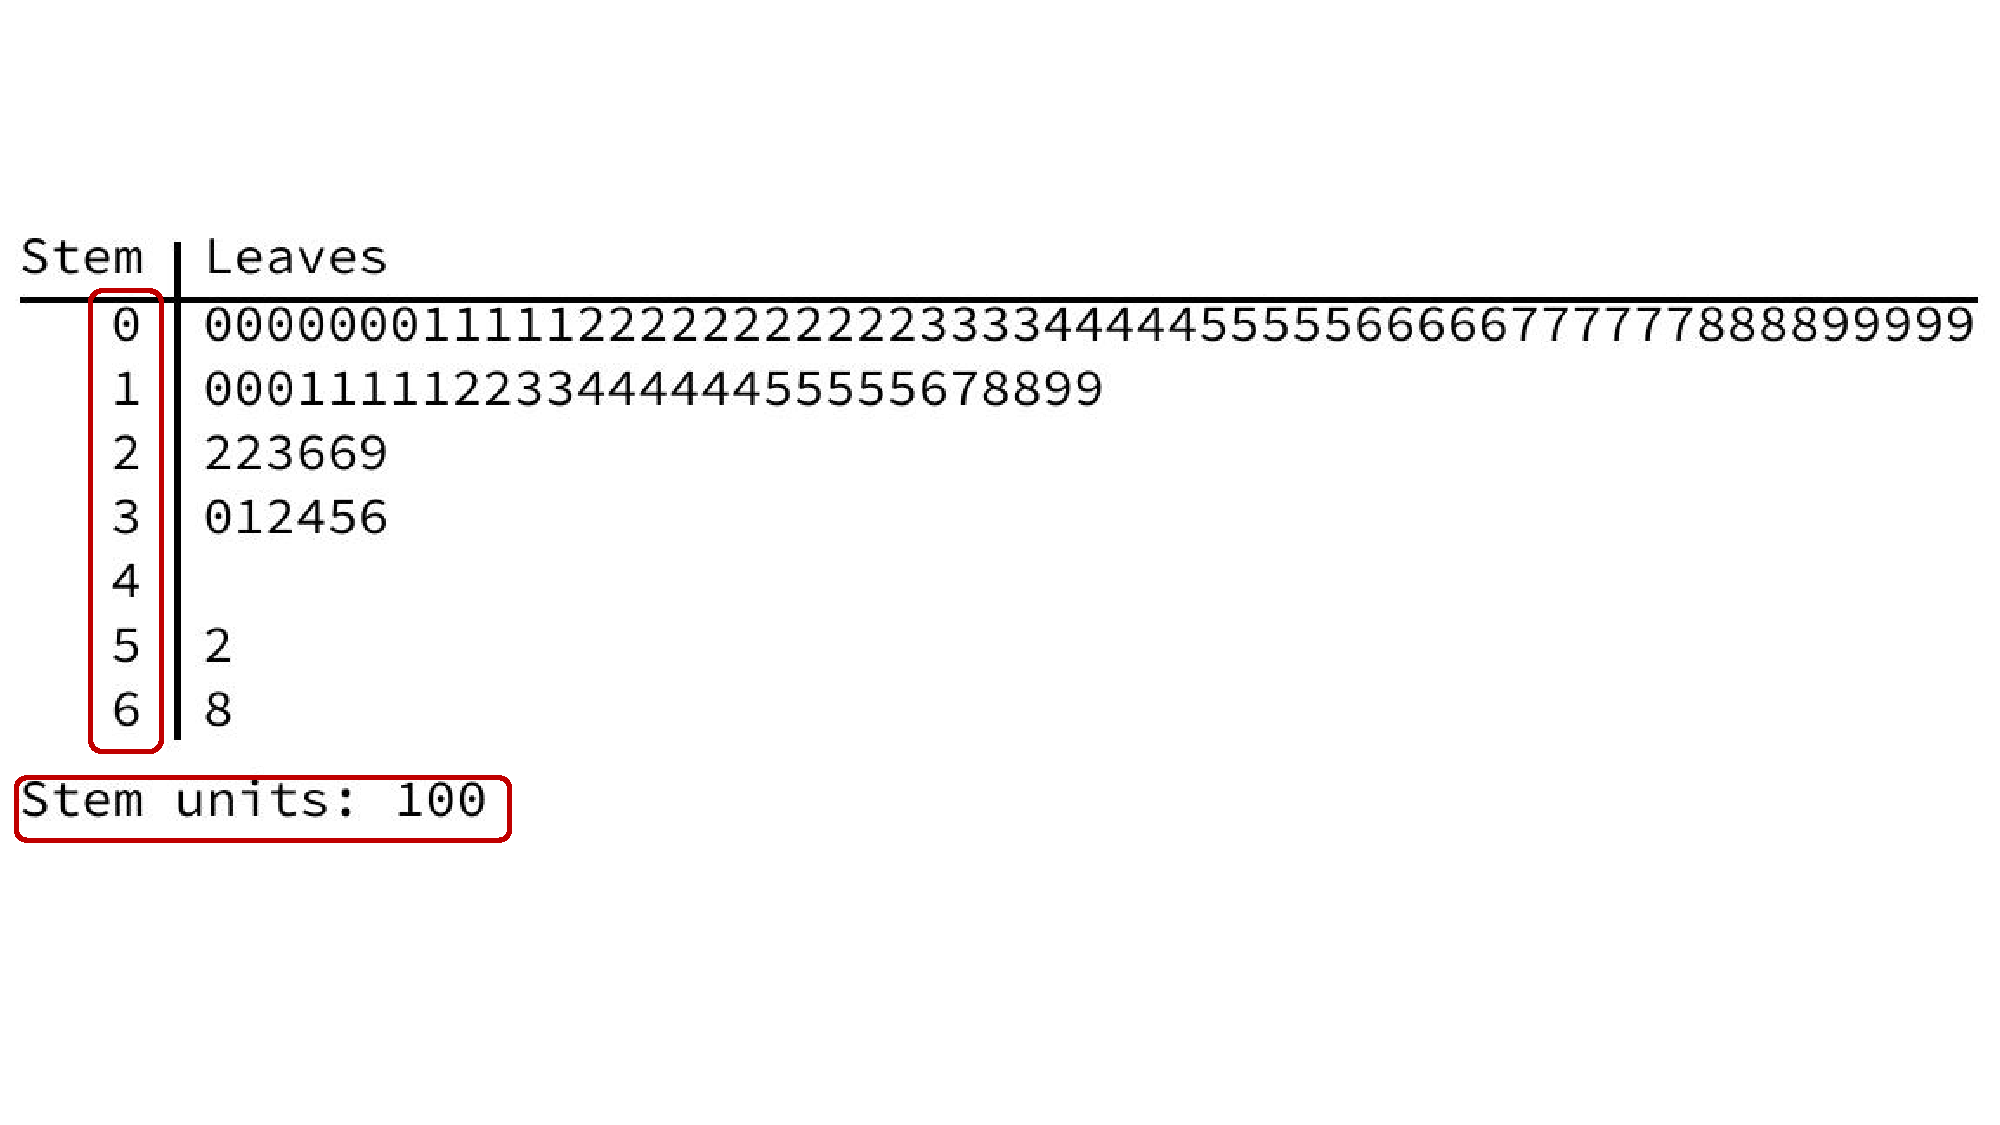
\includegraphics[width=\linewidth]{./images/rc4fig1.pdf}
\end{figure}

\end{frame}


\begin{frame}{Visualization --- Boxplots}

\begin{enumerate}
	\justifying
	\item Calculate $q_1, q_2, q_3$ and $\U{TQR}$.
	\item Find \highlightg{inner fences} and \highlightg{outer fences} by
	\begin{align*}
	& f_1 = q_1 - \frac{3}{2}\U{TQR}, \qquad f_3 = q_3 + \frac{3}{2}\U{IQR}, \\
	& F_1 = q1 - 3\U{IQR}, \qquad F_3 = q_3 + 3\U{IQR},
	\end{align*}
	and find \highlightg{adjacent values}
	\begin{align*}
	a_1 = \min\left\{x_k: x_k\geq f_1 \right\}, \qquad a_3 = \max\{x_k: x_k\leq f_3 \}.
	\end{align*}
	\item Identify \highlightg{near outliers} and \highlightg{far outliers}.
\end{enumerate}

\end{frame}


\begin{frame}{Visualization --- Boxplots}

\begin{figure}[htbp]
	\centering
	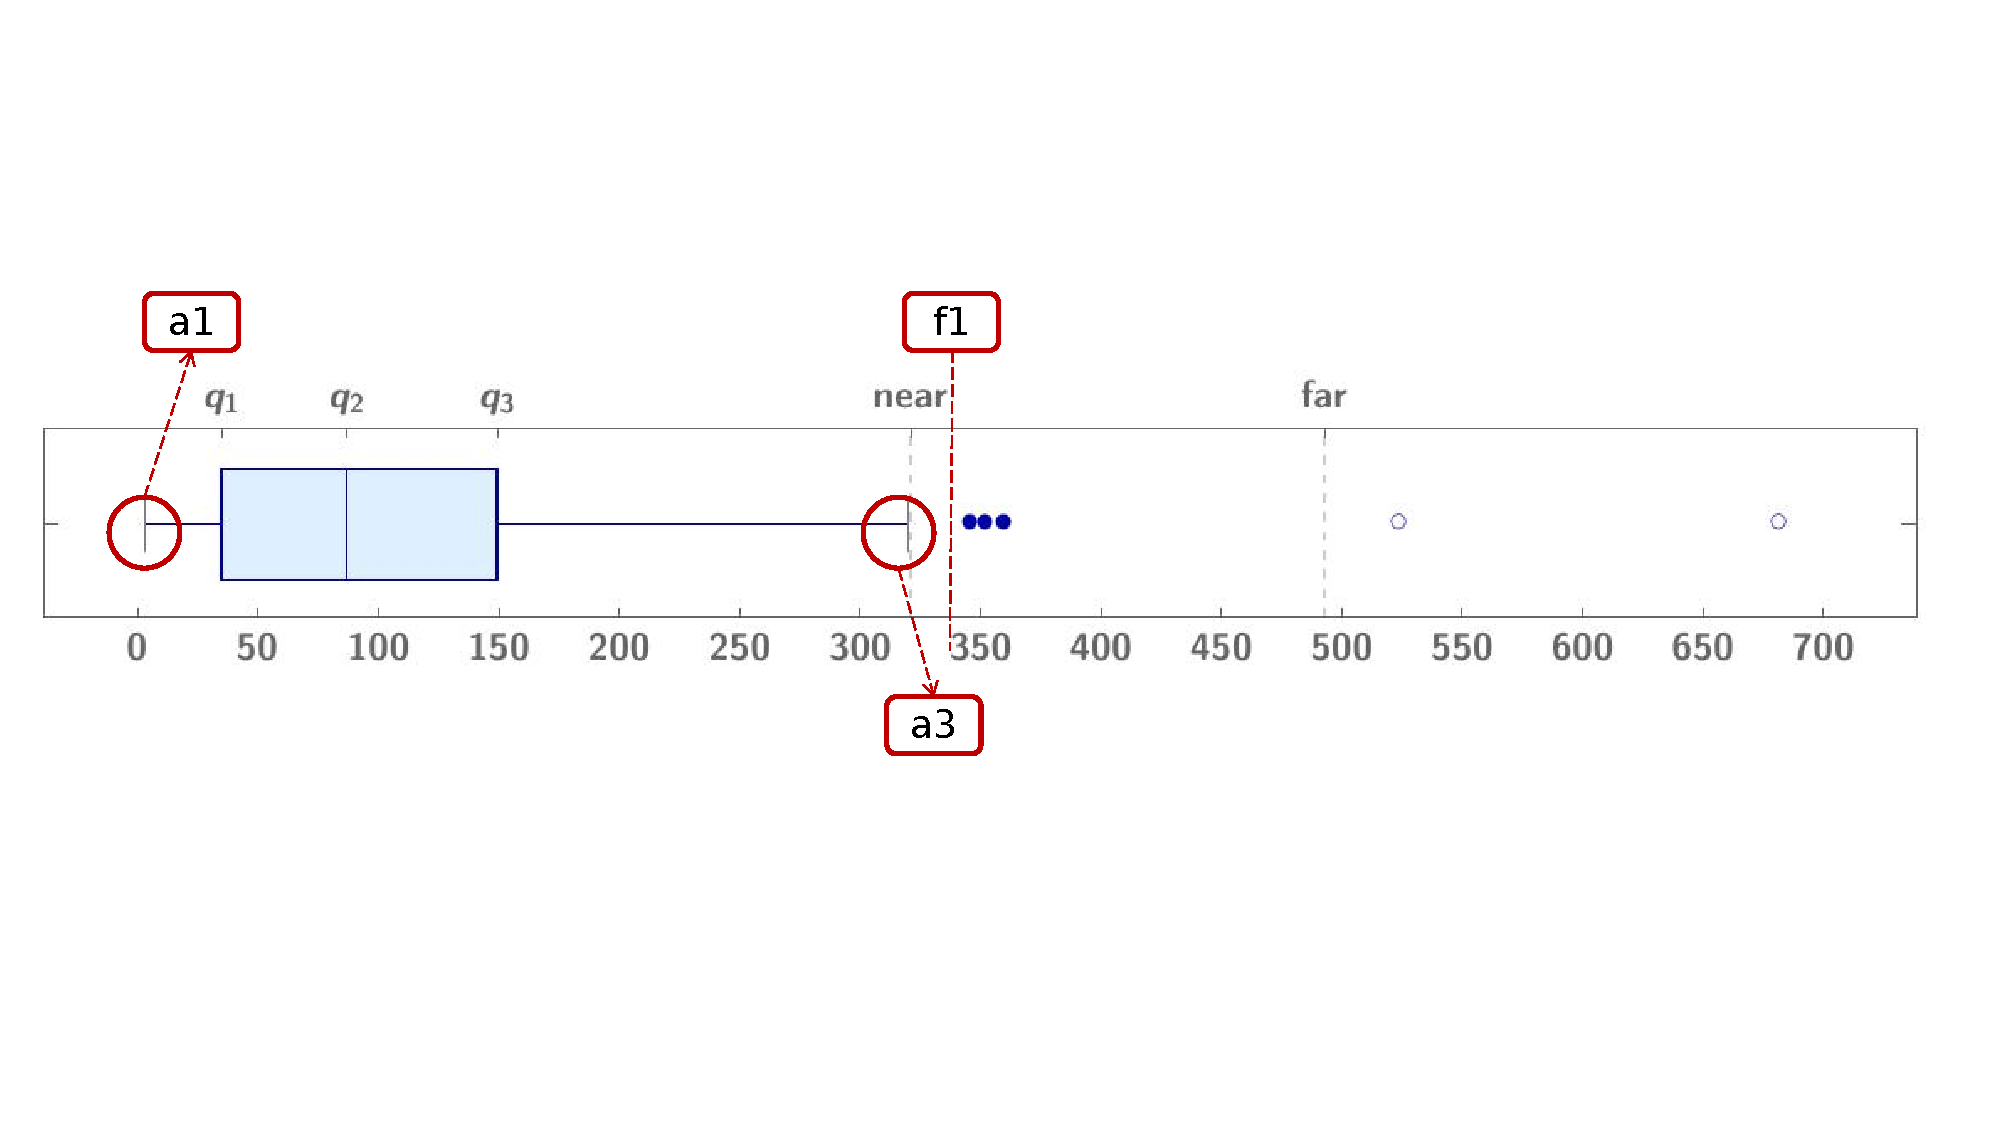
\includegraphics[width=\linewidth]{./images/rc4fig2.pdf}
\end{figure}

\end{frame}


\subsection{Estimating Parameters}

\begin{frame}{Definitions}

\begin{itemize}
	\justifying
	\item \highlightg{Statistic}: a \underline{random variable} that is derived from $X_1, \ldots, X_n$.
	\item \highlightg{Estimator}: a statistic that is used to estimate a population parameter.
	\item \highlightg{Point estimate}: a \underline{value} of the estimator.
	\item \highlightg{Unbiased}: expectation of an estimator $\widehat{\theta}$ is equal to the true parameter.
	\begin{align*}
	\U{E}[\widehat{\theta}] = \theta, \qquad \U{bias} = \theta - \U{E}[\widehat{\theta}].
	\end{align*}
	\item \highlightg{Mean square error}:
	\begin{align*}
	\U{MSE}(\widehat{\theta}) & = \U{E}[(\widehat{\theta} - \theta)^2] \\
	& = \U{E}[(\widehat{\theta} - \U{E}[\widehat{\theta}])^2] + (\theta - \U{E}[\widehat{\theta}])^2 \\
	& = \U{Var}[\widehat{\theta}] + (\U{bias})^2.
	\end{align*}
\end{itemize}

\end{frame}


\begin{frame}{Estimating Parameters --- The Method of Moments}

\justifying
\structb{Method of moments.} Given a random sample $X_1, \ldots, X_n$ of a random variable $X$, for any integer $k\geq 1$, 
\begin{align*}
\widehat{\U{E}[X^k]} = \frac{1}{n}\sum_{i=1}^n X_i^k
\end{align*}
is an unbiased estimator for the $k$th moment of $X$. \\
\structb{Proof.} Denote $\mu_k = \U{E}[X^k]$, then
\begin{align*}
\U{E}\left[\widehat{\mu_k} \right] & = \U{E}\left[\frac{1}{n}\sum_{i=1}^n X_i^k \right] \\
& = \frac{1}{n}\sum_{i=1}^n \U{E}[X_i^k] = \frac{1}{n} \cdot n \mu_k = \mu_k.
\end{align*}


\end{frame}


\begin{frame}{Estimating Parameters --- Method of Maximum Likelihood}

\justifying
\structb{Method of maximum likelihood.} Given a random sample $X_1, \ldots, X_n$ of a random variable $X$ with parameter $\theta$ and density $f_X$, the \highlightg{likeliho-od function} is given by
\begin{align*}
L(\theta) = \prod_{i=1}^n f_{X}(x_i).
\end{align*}
The maximum likelihood estimator (MLE) of $\theta$ is given by
\begin{align*}
\widehat{\theta} = \underset{\theta}{\arg\max}\ L(\theta).
\end{align*}
In most of the cases, we equivalently maximize the \highlightg{log-likelihood}
\begin{align*}
\ell(\theta) = \ln\ L(\theta), \qquad \widehat{\theta} = \underset{\theta}{\arg\max}\ \ell(\theta).
\end{align*}


\end{frame}


\begin{frame}{Estimating Mean}

\structb{Method of moments.}
\begin{itemize}
	\justifying
	\item \underline{Estimating mean $\mu$}.
	\begin{align*}
	\widehat{\mu} = \frac{1}{n}\sum_{i=1}^n X_i.
	\end{align*}
	\item \underline{Biasness}. As we have noted earlier,
	\begin{align*}
	\U{E}\left[\widehat{\mu}\right] = \mu.
	\end{align*}
\end{itemize}

\end{frame}

\begin{frame}{Estimating Mean}

\justifying
\structb{Maximum likelihood estimate}. Suppose $X$ follows a normal distribut-ion with \underline{unknown} mean $\mu$ and \underline{known} variance $\sigma^2$, and we wish to estimate variance $\sigma^2$.
\begin{itemize}
	\item \underline{Estimating variance $\sigma^2$}. 
	\footnotesize
	\begin{align*}
	L(\mu, \sigma^2) & =  \frac{1}{(2\pi)^{n/2}\sigma^n}\exp\left[\frac{1}{\sigma^2}\left(\sum_{i=1}^n X_i^2 - 2\mu\sum_{i=1}^n X_i + n\mu^2 \right) \right]. \\
	\widehat{\mu} & = \underset{\mu}{\arg\max}\left\{-\frac{n}{2}\ln(2\pi\sigma^2) + \frac{1}{\sigma^2}\left(\sum_{i=1}^n X_i^2 - 2\mu\sum_{i=1}^n X_i + n\mu^2 \right) \right\} \\
	& = \frac{1}{n}\sum_{i=1}^n X_i.
	\end{align*}
	\normalsize
	\item \underline{Biasness}. As seen earlier, the estimator is unbiased.
\end{itemize}

\end{frame}


\begin{frame}{Estimating Variance}

\structb{Method of moments}.
\begin{itemize}
	\item \underline{Estimating variance $\sigma^2$}.
	\begin{align*}
	\widehat{\sigma^2} & = \widehat{\U{E}[X^2]} - \widehat{\U{E}[X]}^2 = \frac{1}{n}\sum_{i=1}^n X_i^2 - \left(\frac{1}{n} \sum_{i=1}^n X_i \right)^2.
	\end{align*}
	\item \underline{Biasness}. This estimator is not unbiased since
	\begin{align*}
	\U{E}[X_i^2] & = \U{Var}[X_i] + \U{E}[X_i]^2 = \sigma^2 + \mu^2, \\
	\U{E}[\overline{X}^2] & = \U{Var}[\overline{X}] + \U{E}[\overline{X}]^2 = \frac{\sigma^2}{n} + \mu^2,
	\end{align*}
	and thus
	\begin{align*}
	\U{E}[\widehat{\sigma^2}] = \sigma^2 + \mu^2 - \frac{\sigma^2}{n} - \mu^2 = \frac{n-1}{n}\sigma^2 \neq \sigma^2.
	\end{align*}
\end{itemize}

\end{frame}

\begin{frame}{Estimating Variance}

\justifying
\structb{Maximum likelihood estimate.} Suppose $X$ follows a Poisson distribution with parameter $k$, and we wish to estimate variance $k$ (since both mean and variance of Poisson distribution are $k$).
\begin{itemize}
	\justifying
	\item \underline{Estimating mean $\mu$}. We know from lecture slides that
	\footnotesize
	\begin{align*}
	L(k) & = e^{-nk} \frac{k^{\sum X_i}}{\prod X_i!}, \\
	\widehat{k} & = \underset{k}{\arg\max}\left\{-nk + \ln k\sum_{i=1}^n X_i - \ln\prod_{i=1}^n X_i \right\} \\
	& = \frac{1}{n}\sum_{i=1}^n X_i.
	\end{align*}
	\normalsize
	\item \underline{Biasness}. Although both the MLE estimate for mean and variance are sample mean, the estimators are unbiased.
\end{itemize}

\end{frame}

\begin{frame}{Summary}

\begin{itemize}
	\justifying
	\item \structb{Unbiased estimator for mean and variance.} 
	\begin{align*}
	\widehat{\mu} = \frac{1}{n}\sum_{i=1}^n X_i, \qquad \widehat{\sigma^2} = S^2 = \frac{1}{n-1}\sum_{i=1}^n (X_i - \overline{X})^2.
	\end{align*}
	\item \structb{Unbiased estimator for moments.}
	\begin{align*}
	\widehat{\U{E}[X^k]} = \frac{1}{n}\sum_{i=1}^n X_i^k.
	\end{align*}
	\item \structb{MLE estimator for parameters.}
	\begin{align*}
	\widehat{\theta} = \underset{\theta}{\arg\max}\ \ell(\theta) = \underset{\theta}{\arg\max}\ \sum_{i=1}^n \ln f_{X}(x_i).
	\end{align*}
\end{itemize}


\end{frame}


\subsection{Estimating Intervals}

\begin{frame}{Confidence Intervals}

\justifying
\structb{Definition.} Let $0\leq \alpha \leq 1$. A $100(1-\alpha)\%$ \highlightg{(two-sided) confidence interval} for a parameter $\theta$ is an interval $[L_1, L_2]$ such that
\begin{align*}
P[L_1\leq \theta\leq L_2] = 1 - \alpha.
\end{align*}
In most cases, we use \highlightg{centered confidence interval} with
\begin{align*}
P[\theta < L_1] = P[\theta > L_2] = \frac{\alpha}{2}.
\end{align*}
The $100(1-\alpha)\%$ \highlightg{upper confidence bound} and \highlightg{lower confidence bound} for $\theta$ are given by $L_u, L_l$ such that
\begin{align*}
P[\theta \leq L_u] = 1 - \alpha, \qquad P[L_l \leq \theta] = 1 - \alpha.
\end{align*}

\end{frame}


\begin{frame}{Interval Estimation for Mean and Variance}

\justifying
Suppose we have a random sample of size $n$ from a normal population with \highlightr{unknown} mean $\mu$ and \highlightr{known} variance $\sigma^2$.
\begin{itemize}
	\item \underline{Statistic and distribution}.
	\begin{align*}
	Z = \frac{\overline{X} - \mu}{\sigma / \sqrt{n}} \sim \U{Normal}\left(0, 1 \right).
	\end{align*}
	\item \underline{$100(1-\alpha)\%$ confidence interval for $\mu$}.
	\begin{align*}
	\overline{X} \pm \frac{z_{\alpha/2}\cdot\sigma}{\sqrt{n}}.
	\end{align*}
	\item \underline{$100(1-\alpha)\%$ on-sided interval for $\mu$}.
	\begin{align*}
	L_u = \overline{X} + \frac{z_{\alpha}\cdot\sigma}{\sqrt{n}}, \qquad L_l = \overline{X} - \frac{z_{\alpha}\cdot \sigma}{\sqrt{n}}.
	\end{align*}
\end{itemize}

\end{frame}


\begin{frame}{Interval Estimation for Mean and Variance}

\justifying
Suppose we have a random sample of size $n$ from a normal population with \highlightr{unknown} mean $\mu$ and \highlightr{unknown} variance $\sigma^2$.
\begin{itemize}
	\item \underline{Statistic and distribution}.
	\begin{align*}
	Z = \frac{\overline{X} - \mu}{\sigma / \sqrt{n}} \sim \U{Normal}\left(0, 1 \right).
	\end{align*}
	\item \underline{$100(1-\alpha)\%$ confidence interval for $\mu$}.
	\begin{align*}
	\overline{X} \pm \frac{z_{\alpha/2}\cdot\sigma}{\sqrt{n}}.
	\end{align*}
	\item \underline{$100(1-\alpha)\%$ on-sided interval for $\mu$}.
	\begin{align*}
	L_u = \overline{X} + \frac{z_{\alpha}\cdot\sigma}{\sqrt{n}}, \qquad L_l = \overline{X} - \frac{z_{\alpha}\cdot \sigma}{\sqrt{n}}.
	\end{align*}
\end{itemize}

\end{frame}
